\documentclass[10pt,a4paper]{article}

\usepackage[utf8]{inputenc}
\usepackage[T1]{fontenc}
\usepackage[margin=1.45cm]{geometry}
\usepackage{amsmath}
\usepackage{array}
\usepackage{booktabs}
\usepackage{tabularx}
\usepackage{graphicx}
\usepackage{float}
\usepackage{caption}
\usepackage{xcolor}
\usepackage{tikz}
\usetikzlibrary{arrows.meta,positioning,shapes.geometric,fit}
\usepackage{tcolorbox}
\usepackage{hyperref}

\hypersetup{colorlinks=true,linkcolor=black,urlcolor=blue}
\setlength{\parindent}{0pt}
\setlength{\parskip}{3pt}
\captionsetup{font=footnotesize,labelfont=bf}
\newcolumntype{Y}{>{\raggedright\arraybackslash}X}

\definecolor{riverblue}{HTML}{1F5A85}
\definecolor{waterlight}{HTML}{EAF4FA}
\definecolor{actiongreen}{HTML}{EAF5E9}
\definecolor{warningorange}{HTML}{FFF3DD}
\definecolor{riskred}{HTML}{FBEAEA}
\definecolor{ink}{HTML}{203040}

\title{\vspace{-1.0cm}\textbf{Decision Brief: Fish, Warming and Barriers in the Guadalquivir Basin}}
\author{\textit{A practical summary for basin managers and decision makers}}
\date{September 2026}

\begin{document}
\maketitle
\vspace{-0.5cm}

\begin{tcolorbox}[colback=riverblue!9,colframe=riverblue!70!black,title=\textbf{The decision in one minute},fonttitle=\bfseries]
The simulations do not support a single basin-wide rule of ``remove all barriers'' or ``keep all barriers''. They show that the effect of a barrier depends on the network around it and on invasive-species pressure. The most immediate warming signal is a decline in cold-water brown trout, not a rapid loss of total fish richness. Management should therefore combine three actions: protect cool headwater refuges, assess barrier projects at local network scale, and pair connectivity improvements with invasive-species control.
\end{tcolorbox}

\section*{What was assessed?}

The analysis represents 775 sites and 24 fish species across the Guadalquivir River Basin. It follows daily water temperature and fish movement through a branching river network from 2026 to 2045. It compares 44 climate combinations, a no-warming control, 32 barrier and movement scenarios, and 48 interaction scenarios. Results are designed to compare management choices and mechanisms, not to provide a precise extinction forecast.

\begin{figure}[H]
\centering
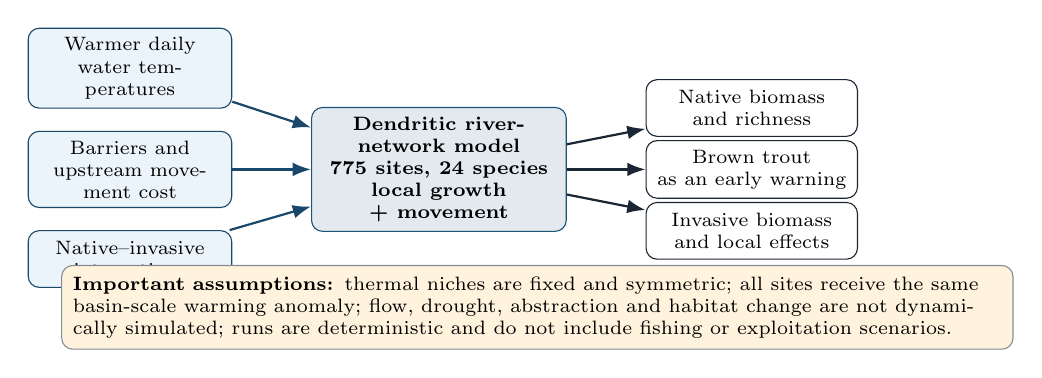
\begin{tikzpicture}[>=Latex, node distance=0.28cm and 0.45cm, every node/.style={font=\scriptsize},
  input/.style={draw=riverblue!80!black, fill=waterlight, rounded corners, align=center, text width=2.35cm, minimum height=0.72cm},
  model/.style={draw=riverblue!90!black, fill=riverblue!13, rounded corners, align=center, text width=3.0cm, minimum height=1.15cm, font=\scriptsize\bfseries},
  output/.style={draw=ink!80!black, fill=white, rounded corners, align=center, text width=2.45cm, minimum height=0.72cm},
  note/.style={draw=ink!55, fill=warningorange, rounded corners, align=left, text width=11.8cm, inner sep=4pt}]
\node[input] (heat) {Warmer daily\\water temperatures};
\node[input, below=of heat] (barrier) {Barriers and\\upstream movement cost};
\node[input, below=of barrier] (biotic) {Native--invasive\\interactions};
\node[model, right=1.0cm of barrier] (model) {Dendritic river-network model\\775 sites, 24 species\\local growth + movement};
\node[output, right=1.0cm of model, yshift=0.78cm] (native) {Native biomass\\and richness};
\node[output, right=1.0cm of model] (trout) {Brown trout\\as an early warning};
\node[output, right=1.0cm of model, yshift=-0.78cm] (inv) {Invasive biomass\\and local effects};
\draw[->, thick, riverblue!80!black] (heat) -- (model);
\draw[->, thick, riverblue!80!black] (barrier) -- (model);
\draw[->, thick, riverblue!80!black] (biotic) -- (model);
\draw[->, thick, ink!80!black] (model) -- (native);
\draw[->, thick, ink!80!black] (model) -- (trout);
\draw[->, thick, ink!80!black] (model) -- (inv);
\node[note, below=0.42cm of model, xshift=1.25cm] {\textbf{Important assumptions:} thermal niches are fixed and symmetric; all sites receive the same basin-scale warming anomaly; flow, drought, abstraction and habitat change are not dynamically simulated; runs are deterministic and do not include fishing or exploitation scenarios.};
\end{tikzpicture}
\caption{\textbf{How to read the evidence.} The model links the three pressures that managers can influence or monitor to outcomes for native fish, brown trout and invasive fish. The assumptions define the limits of the conclusions.}
\end{figure}

\clearpage
\section*{Three findings that matter for decisions}

\begin{tcolorbox}[colback=actiongreen,colframe=green!45!black,title=\textbf{1. Protect cold-water refuges now},fonttitle=\bfseries]
Brown trout biomass fell by 9--11\% across the warming scenarios, compared with 0.2\% in the no-warming control. The decline was accompanied by more days above the trout upper thermal limit. This is the clearest early warning in the basin model. Protect headwaters, high-elevation reaches, riparian shade and reliable summer refuges even though basin-wide richness changes little.
\end{tcolorbox}

\begin{tcolorbox}[colback=warningorange,colframe=orange!60!black,title=\textbf{2. Assess every barrier in its network context},fonttitle=\bfseries]
The effect of blocking a barrier changed from negative to positive as background upstream movement cost increased. This does not mean that blocking barriers is beneficial. It means that the same intervention can have different outcomes depending on the surrounding network, native rescue routes and invasive dispersal. Evaluate proposed removal, passage improvement or restriction at reach and sub-catchment scale, not from the basin average alone.
\end{tcolorbox}

\begin{tcolorbox}[colback=riskred,colframe=red!55!black,title=\textbf{3. Pair connectivity work with invasive control},fonttitle=\bfseries]
In the deliberately strong invasive-favouring scenario, native biomass fell by about 90\% while invasive biomass increased almost tenfold and total biomass changed much less. This is a warning about structural risk, not a prediction. Where passage is improved, strengthen surveillance and control of invasive fish at likely source reaches and reservoirs.
\end{tcolorbox}

\begin{figure}[H]
\centering
\includegraphics[width=\textwidth,height=0.78\textheight,keepaspectratio]{../results/sensitivity_obstacles/report_plots/fig_passability_uc_heatmaps.png}
\caption{\textbf{How a barrier effect depends on the surrounding network.} Change in each response metric caused by altering obstacle passability, measured against the baseline-passability run for the same model and upstream cost. Within every panel the rows are the four passability states (baseline, improved, reduced, blocked) and the columns are the four upstream movement costs (0.01, 0.05, 0.10, 0.50). Panels are arranged as four rows of metrics and two columns of climate endpoints: (a) cool and (b) warm for total biomass, (c) cool and (d) warm for native biomass, (e) cool and (f) warm for native richness, and (g) cool and (h) warm for brown-trout (ST) final biomass. The cool endpoint is SSP1-2.6/IITM-ESM and the warm endpoint is SSP2-4.5/UKESM1. Each cell states the raw difference in model units (the baseline row is zero by construction); its colour is that difference divided by the panel's 95th percentile, so colours compare within a panel but not between panels. In the native-biomass row (c, d), blocking and reducing passability move from negative at low cost to positive at high cost, whereas improving passage is negative at every cost. This supports site-specific assessment; it does not identify barrier construction as a conservation action.}
\end{figure}

\begin{figure}[H]
\centering
\includegraphics[width=\textwidth,height=0.72\textheight,keepaspectratio]{../results/climate_scenarios_k1x_burnin/figures/report_plots/fig12_st_climate_response.png}
\caption{\textbf{Warming sentinel: brown trout.} Each point is one climate-model/pathway run (11 GCMs $\times$ 4 pathways) plotted against the imposed basin-mean warming by 2045; the black diamond is the no-warming control. Panel (a): relative change in basin brown trout (ST) biomass as a percentage of its spun-up baseline, with the dashed ordinary-least-squares fit of about $-9.2$\% per $^\circ$C ($R^2=0.65$). Panel (b): absolute final ST biomass in model units. Panel (c): maximum number of days per year above the species' 20~$^\circ$C upper thermal limit, with the control value (131 days) as a dotted reference line. Brown trout declines consistently with warming while thermal exposure rises, so species-level monitoring detects change that aggregate richness misses.}
\end{figure}

\clearpage
\section*{Where should action be targeted?}

The positive basin-level effect of blocking at high upstream cost is not uniform. Some sub-catchments and water bodies gain native biomass while others lose it. Decisions should therefore be made with local maps of native refuges, invasive distributions, barrier position and movement cost.

\begin{figure}[H]
\centering
\includegraphics[width=\textwidth,height=0.78\textheight,keepaspectratio]{../results/sensitivity_obstacles/report_plots/fig_subcatchment_waterbody_effects.png}
\caption{\textbf{Local gains and losses hidden by the basin average.} Blocked-minus-baseline change in native biomass (model units) for the warm endpoint, high upstream cost and year 2045. Panel (a) shows the 10 most negative and 10 most positive of the 77 sub-catchments (20 bars); panel (b) shows the 10 most negative and 10 most positive of the 289 water bodies (20 bars). Bars are sorted from most negative to most positive; red bars are losses and green bars are gains. The basin-mean effect is a net of both signs, so a positive average must not be read as a uniform benefit to native fish; decisions belong at sub-catchment or water-body scale.}
\end{figure}

\begin{center}
\small
\begin{tabularx}{0.98\textwidth}{>{\raggedright\arraybackslash}p{0.26\textwidth}YY}
\toprule
Management question & Evidence from the simulations & Practical response \\
\midrule
Where should passage be improved? & Where native rescue is limited, invasive pressure is low, and cool refuges remain connected. & Prioritise local projects after reach-level assessment; do not use a basin-wide average as the sole criterion. \\
What should accompany passage improvement? & Increased movement can redistribute both native and invasive biomass. & Add invasive surveillance, rapid response, and source-population control to passage projects. \\
Where should warming adaptation start? & Trout responds strongly while aggregate richness is nearly flat. & Monitor cold-water specialists and protect headwater and shaded reaches. \\
What should be avoided? & The model does not simulate drought, flow change or extinction probability. & Do not treat these results as a standalone legal status assessment or an extinction forecast. \\
\bottomrule
\end{tabularx}
\end{center}

\clearpage
\section*{A practical management plan}

\begin{enumerate}
\item \textbf{Protect and monitor thermal refuges.} Establish a basin network of cold-water sentinel reaches. Record summer temperature, days above species limits, trout occupancy and abundance, riparian shade and local flow persistence.
\item \textbf{Screen connectivity projects locally.} For each barrier, map upstream movement cost, connected native populations, invasive presence, downstream sources and the possibility of local redistribution. Compare removal, fish passage, partial passage and no-action alternatives.
\item \textbf{Make invasive management part of connectivity policy.} Treat new passage as a coupled restoration-and-biosecurity project. Monitor upstream spread after intervention and target high-risk source reaches before construction.
\item \textbf{Use aggregate indicators carefully.} Basin richness and total biomass are useful broad indicators, but they can remain stable while a rare cold-water specialist declines. Report species-level trends alongside basin means.
\item \textbf{Update the assessment as hydrology changes.} The present model isolates temperature, network movement and interactions. Future decision support should add discharge, drought, abstraction, habitat degradation and exploitation before quantitative investment ranking.
\end{enumerate}

\begin{tcolorbox}[colback=waterlight,colframe=riverblue!70!black,title=\textbf{What this evidence does and does not say},fonttitle=\bfseries]
\textbf{It does say:} network resistance and interaction structure can control aggregate outcomes; brown trout is an early warming indicator; barrier effects are context dependent; and native and invasive biomass can be redistributed without much change in total biomass.

\textbf{It does not say:} that warming causes basin-wide extinction by 2045; that every barrier should be retained or removed; that a positive basin mean benefits every reach; or that the extreme invasive-favouring scenario is a forecast.
\end{tcolorbox}

\vfill
\begin{center}
\footnotesize
\textit{Evidence basis: deterministic spatial simulations of 775 sites and 24 fish species for 2026--2045, including 44 climate scenarios, a no-warming control, 32 obstacle scenarios and 48 interaction-structure scenarios. Full methods, figures and references are provided in the accompanying technical report.}
\end{center}

\end{document}
